%%
%% This is file `cimsmple.tex',
%% generated with the docstrip utility.
%%
%% The original source files were:
%%
%% cimento.dtx  (with options: `sample')
%% 
%% IMPORTANT NOTICE:
%% 
%% For the copyright see the source file.
%% 
%% Any modified versions of this file must be renamed
%% with new filenames distinct from cimsmple.tex.
%% 
%% For distribution of the original source see the terms
%% for copying and modification in the file cimento.dtx.
%% 
%% This generated file may be distributed as long as the
%% original source files, as listed above, are part of the
%% same distribution. (The sources need not necessarily be
%% in the same archive or directory.)
%%%%%%%%%%%%%%%%%%%%%%%%%%%%%%%%%%%%%%%%%%%%%%%%%%
%%%%%%%%%%%%%%%%%%%%%%%%%%%%%%%%%%%%%%%%%%%%%%%%%%
%%%%%%%%%%%%%%%%%%%%%%%%%%%%%%%%%%%%%%%%%%%%%%%%%%
\ProvidesFile{cimsmple.tex}
      [1999/12/01 v1.4c Il Nuovo Cimento]
\documentclass{cimento}

\usepackage{epsfig}
%%%%%%%%%%%%%
             %
               %    % If you are preparing Enrico Fermi School of
%VERY IMPORTANT  %  % Physics report, please read the bundled file
	       %    % README.varenna 
             %
%%%%%%%%%%%%


%\usepackage{graphicx}  % got figures? uncomment this
\title{Top physics beyond the standard model: Prospects at CMS}
\author{Francisco~Yumiceva (for the CMS Collaboration)\from{ins:x}}
\instlist{\inst{ins:x} Fermi National Accelerator Laboratory, Batavia, Illinois, USA}
\PACSes{\PACSit{14.65Ha}{top quarks.}}
\begin{document}

\maketitle

\begin{abstract}
Precise studies of the top-quark sector will be performed in the LHC
in order to test the standard model and search for new physics.
The top-quark sector at the LHC opens a very rich region to look for new 
phenomena. Searches beyond the standard model include new top quark 
decays 
and top quarks in resonant production. In the latter, a good observable to carry on a 
model-independent 
search is the top pair invariant mass. A special reconstruction
procedure is needed for the case of heavy resonances decaying into very
high-$p_{T}$ top jets. 
CMS is developing tools to improve 
the reconstruction of these highly boosted top jets and studying the discovery potential for new physics in the top quark sector. A brief review of these studies
is given in this note.
\end{abstract}

\section{Introduction}
\label{sec:Intro}

Precision top-quark physics will be carried on by the LHC experiments
thanks to production of a much larger data set than the current Tevatron top-quark sample.
At the design luminosity of $10^{-34}$~cm$^{-2}$s$^{-1}$, the LHC will
produce about 80 million top pairs and 40 million single top events per
year. The large statistics top event sample opens the possibility to use top quark
events as a tool to calibrate the detector. For example, top quark events
can be used to measure the absolute jet energy scale and 
the $b$-tagging efficiency. Besides testing the standard model (SM) and using top
events as a standard candle, top physics opens a rich region for searches
beyond the standard model (BSM). Because of the large top Yukawa coupling,
we expect new physics to have strong couplings to the top sector~\cite{ref:Wang}.
New phenomena in the top-quark sector can appear as new
decay channels or top quarks in resonant production~\cite{ref:Han}.

The top quark has a special role both in the standard model and BSM. Within
the SM, the top quark is naturally related to the electroweak (EWK)
symmetry breaking (EWSB) because of its large Yukawa coupling to the SM Higgs,
and because the top mass is at the EWK scale. In addition, the top-quark loop
presents the largest contribution to the quadratic divergence of
the SM Higgs mass. Because of its prompt decay, it offers the possibility to study 
properties of a bare quark, {\it e.g.} spin, mass, and coupling. Within 
BSM models, there are many alternative mechanisms of EWSB, {\it e.g} models with top partners
in order to compensate for the large top radiative correction to the Higgs 
mass (SUSY, Little Higgs, Extra Dimensions). The large top mass opens up
a large phase space for decays to heavy states. There are models where couplings
of new gauge interactions to the top quark are enhanced. In such models new particles 
could show up as resonances which decay to $t\bar{t}$. 

In this note, we summarize the results of exploring the discovery
potential in the top sector with the CMS detector. A detail description
of the CMS detector can be found somewhere else~\cite{ref:CMS}. We concentrate
on searches for new top decays and the search for heavy resonances into
$t\bar{t}$ decays. Studies about the search for top partners and other exotic
top searches are currently being done in CMS.

\section{Top quark decays}
\label{sec:Decays}

In the SM, flavor changing neutral currents (FCNC) are suppressed by
the GIM mechanism. The dominant decay channels are through the
weak charged-currents (CC). Because of $V_{tb}>>V_{td},V_{ts}$~\cite{ref:pdg}, the 
predominant top decay channel is to a $b$ quark. In addition, the top
quark has a prompt decay via the first order weak interaction which
occurs before
hadronization,  $\Gamma(t\rightarrow W^+ q) \approx 1.5$~GeV $> \Lambda_{QCD}
 \sim 200$~MeV.
 

\begin{figure}
\centering
\includegraphics[width=0.4\textwidth]{fig01a.ps}
\includegraphics[width=0.49\textwidth]{fig01b.ps}
\caption{(a) Branching ratio of $t\rightarrow H^{\pm}b$ vs $\tan \beta$,
and (b) branching ratios for charged Higgs boson decaying to different final
states for $\tan \beta=20$.}
\label{fig:fig1}
\end{figure}



\subsection{Top charged current decays in BSM}
\label{sec:CC}

Alternative top quark CC decays are possible via charged technicolor
particles, {\it e.g.} $t\rightarrow \pi^+_{T}b$,  and charged Higgs in 
Supersymmetry (SUSY) or with an extended Higgs sector $t\rightarrow H^{+}b$. 
The former
decay channel has not been explored yet by CMS. The latter decay channel
could be the leading channel for charged Higgs production. CMS has
explored the discovery potential of this decay in the context
of the minimal supersymetric model (MSSM). A more detailed
description of this analysis can be found in the ref.~\cite{ref:ptdr2}.
The branching ratio of top to a charged Higgs boson depends on both its
mass and $\tan \beta$ as shown in fig.~\ref{fig:fig1}(a). For $\tan \beta=20$,
the charged Higgs boson mostly decays to $\tau \nu$ for $m_{H^{\pm}}<m_{t}$ where
$m_{t}$ is the top mass [see fig.~\ref{fig:fig1}(b)]. For $m_{H^{\pm}}>m_{t}$, 
the two main decay modes are to $tb$ or $\tau \nu$ as shown in fig.~\ref{fig:fig1}(b).
Therefore, we can study the following main final states:

\begin{itemize}
\item If $m_{H^{\pm}}<m_{t}$, $t\bar{t}\rightarrow H^{\pm}W^{\mp}b\bar{b}\rightarrow (\tau^{\pm}\nu)(l^{\mp}\nu)b\bar{b}$.
\item If $m_{H^{\pm}}>m_{t}$, $gg\rightarrow tbH^{\pm}\rightarrow (j_{1}j_{2})(bb(\tau^{\pm}\nu))$.
\item If $m_{H^{\pm}}>m_{t}$, $gb\rightarrow tH^{\pm} \rightarrow ttb \rightarrow W^+W^-bbb\rightarrow j_1j_2\mu\nu bbb$ and $gg\rightarrow tH^{\pm}b \rightarrow ttbb \rightarrow W^+W^-bbbb\rightarrow j_1j_2\mu\nu bbbb$.
\end{itemize}

  


The final state $(\tau^{\pm}\nu)(l^{\mp}\nu)b\bar{b}$ was studied using fully
simulated data, including pile-up, corresponding to a low luminosity of 
$2\times10^{33}$~cm$^{-2}$s$^{-1}$~\cite{ref:tauLepAna}. The Level-1 (L1) trigger and High Level Trigger (HLT) selection
includes a single muon, $p_{T}>20$~GeV/c, and an electron, $p_{T}>30$~GeV/c.
The offline reconstruction uses jets with $E_{T}>40$~GeV/c. The jet
algorithm uses the iterative jet cone reconstruction with $\Delta R=0.5$.
Jets are required to be central $| \eta_{jet}|<2.4$. At least three jets are
required in the event and at least one of the jets tagged as a $b$-jet. The 
$b$-tagging algorithm is based on the impact parameter significance of tracks in the jet.
The on-line tau reconstruction at L1 requires tau-like energy deposits 
in the calorimeters. Regional jet reconstruction around the L1 tau candidate
is performed with $E_{T}>20$~GeV/c. Electron fakes are reduced by requiring
that the most energetic hadron calorimeter tower have $E_{T}>2$~GeV. Then, the tau offline
reconstruction follows using three concentric cones to identify tau candidates.
Tau jet candidates are required to have $E_{T}>40$~GeV. The total charge of the
lepton plus the tau jet is required to be zero. To reduce background,
the missing transverse energy (MET) has to be greater than 70~GeV. The main 
background channels are QCD $t\bar{t}$ with at least a single electron or muon
tau jets, W+jets, and single top. The total systematic uncertainty is 
around 5\%, where the main contributions come from $b$-tagging and tau identification.
The 5$\sigma$ discovery potential for a light $H^{\pm}$ boson at 30~$fb^{-1}$
integrated luminosity including the effect of systematic uncertainties is shown in fig.~\ref{fig:fig2}.


\begin{figure}
\centering
\includegraphics[width=0.6\textwidth]{fig02.ps}

\caption{Discovery potential (5$\sigma$) for light charged Higgs boson with
30~$fb^{-1}$ including the effect of systematic uncertainties.}
\label{fig:fig2}
\end{figure}

 
The final state $(j_{1}j_{2})bb(\tau^{\pm}\nu)$ has also been studied in 
CMS~\cite{ref:jjtauAna}. Fully
simulated data at low luminosity was used in this analysis. The main background
channels are tau decays from QCD $t\bar{t}$, and taus from W decays. We can take 
advantage in this channel of the large MET for $H^{\pm}$ decays. The reconstruction
of the top mass helps to suppress QCD multi-jet background. In addition, helicity
correlations favoring $H^{+}$ decays over W decays due to the spin-parity
properties of the decaying particles are employed. The main systematic uncertainties arise from
tau identification, $~8$\%, and the $t\bar{t}$ background, about 11\%. For the
other backgrounds, the MC statistics strongly dominate the measurement uncertainties
and therefore the MC statistics uncertainties were used. Fig.~\ref{fig:fig3} shows
the 5$\sigma$-discovery region in the $m_{A}-\tan \beta$ plane.


\begin{figure}
\centering
\includegraphics[width=0.6\textwidth]{fig03.ps}

\caption{Discovery potential (5$\sigma$) for the channel $gg\rightarrow tbH^{\pm}\rightarrow (j_{1}j_{2})(bb(\tau^{\pm}\nu))$ at 30~$fb^{-1}$ in the maximal mixing scenario with
$\mu = 200$~GeV/c$^{2}$. The discovery regions with and without systematic uncertainties
are shown. The regions excluded by LEP and Tevatron searches are also shown.}
\label{fig:fig3}
\end{figure}


The final states $j_1j_2\mu\nu bbb$ and $j_1j_2\mu\nu bbbb$ are the most interesting
from the experimental point of view because an isolated muon is present which will satisfy the CMS
trigger and the branching fraction into this decay is high~\cite{ref:jetsAna}.
The production of $H^{+}$ through heavy SUSY particles is not taken into account.
The main background in these channels is $t\bar{t}+jets$. The selection includes
a single muon trigger, $p_{T}>20$~GeV/c, at least 5(6) jets with
$E_T>25$~GeV, and at least 3(4) $b$-tagged jets. The secondary vertex algorithm
is used to identify $b$-jets. The best jet association is based on a likelihood
ratio which contains information from the kinematic variables of jets, output of
a kinematic fit on the $t\bar{t}$ system with a W and top mass constraint, and
$b$-tagging discriminants. The largest systematic uncertainty is in the 
estimation of the large background. Even with a very optimistic analysis at an integrated luminosity of
30~$fb^{-1}$ no visibility for these channels is obtained within the MSSM. The
discovery contours for both final states are shown in fig.~\ref{fig:fig4}.


\begin{figure}
\centering
\includegraphics[width=0.49\textwidth]{fig04a.ps}
\includegraphics[width=0.49\textwidth]{fig04b.ps}
\caption{Discovery contours for $H^{\pm}\rightarrow tb$ decay for 30~$fb^{-1}$
with a three $b$-jet final state (a)$j_1j_2\mu\nu bbb$, and a four $b$-jet final state
(b)$j_1j_2\mu\nu bbbb$. The systematic uncertainty shown is due to
estimated background leakage efficiencies of 0\%, 1\%, and 3\%.}
\label{fig:fig4}
\end{figure}


\subsection{Top neutral current decays in BSM}
\label{sec:FCNC}

Within SUSY, we can have new decay modes like $t\rightarrow\tilde{t}\tilde{\chi}^0$.
These decays modes have not been explored in CMS. The decays explored are
due to FCNC at loop level which are highly suppressed in the SM with branching
fractions about $10^{-14}$. Within the MSSM, we can have branching fractions of
about $10^{-5}$. The possible decays are $t\rightarrow \gamma+jet$, 
$t\rightarrow Z+jet$, and $t\rightarrow g+jet$. The last channel has not
been studied because of the very high background. The analyses look for one SM
top decay and another FCNC decay. Only the muon and electron decays from W and Z
are studied. The main background sources are QCD $t\bar{t}$, single top (t-channel),
ZW+jets, WW+jets, ZZ+jets, W+jets, Z+jets, Z$b\bar{b}$, and QCD. A detailed description of these analysis
can be found in ref.~\cite{ref:ptdr2}.


\section{Top quarks in resonant production}
\label{sec:Resonances}

In the SM at $E_{cm}=14$~TeV, top quarks are produced via QCD production by the fusion of $q\bar{q}$ (10\%) and
$gg$ (90\%), via single top production, and via Higgs associated production $t\bar{t}H$.
Beyond the SM, top quarks can also be produced in resonant production. In many models, there is
a high potential to discover new physics in the top quark sector by searching for
heavy resonances which decay into $t\bar{t}$ or $t\bar{b}$. Resonant states 
include Higgs bosons, new gauge bosons, Kaluza-Klein excitations of gluons and
gravitons, technicolor-like dynamical states. New phenomena can
be observed in the $m_{t\bar{t}}$ distribution as shape distortions or peaks. The distortions
can be deviations of the distribution from the theoretical predictions due to enhancements
or interferences of new physics~\cite{ref:Maltoni}. Therefore, the $m_{t\bar{t}}$
distribution is a good observable and CMS will use it to carry on a model independent search. The
$m_{t\bar{t}}$ distribution can be divided in three regions (see fig.~\ref{fig:fig5}). The low mass region, 
between 300 to 800~GeV/c$^2$, is where most of the SM background peaks and the
standard tools to reconstruct top quark events can be applied. The medium region,
between 800 to 1000~GeV/c$^2$, is where the standard tools begin to have low efficiency
and a special reconstruction approach is needed to recover efficiency. The high
mass region, above 1~TeV/c$^2$, is where the top quark is highly boosted. The decay
products can be merged and the reconstruction of these objects requires a different approach.
However, the event topology of these decays and the presence of high-$p_T$ jets can help
to reconstruct these special decays.

We are studying new techniques to improve the reconstruction of highly boosted top jets. The 
main problem with these events is that the decay products of the top jet are very close to each other.
In fig.~\ref{fig:fig7}(a), the lego plot of the calorimeter towers of the
four leading jets is shown from a sample of muonic QCD $t\bar{t}$. In fig.~\ref{fig:fig7}(a) is possible to 
easily distinguish two $b$-jets and two light jets from the W decay. In fig.~\ref{fig:fig7}(b),
the lego plot is shown for the case of a narrow resonance $Z'(4~TeV)\rightarrow t\bar{t}$.
The top jet products are all merged into a high-$p_T$ jet, and a second jet with lower $p_T$ opposite to the
leading jet. The most simple method to reconstruct these merged jets is to use a jet 
association based in $\Delta R$. The leading jet is selected and the rest of jets around this
jet are added vectorially to the leading jet. Then, the mass of this new merged jet (MJet) is obtained which
has a mass near the top mass. An additional selection can be applied using topology variables, {\it e.g.} requiring
that the merged jet be opposite to the second jet. The use of the variable $\Delta R$ is not
suitable because of its strong dependency on the center of mass decay angle of the top. This produces
distortions of the angular distributions and hence the possible spin determination of the parent resonance. A new
variable called $\psi$ has been studied to replace $\Delta R$. The variable $\psi$ is inspired by
the $k_T$ jet algorithm. Given a particle of mass $M$ which has a
two-body decay to particles of momentum $p_1$ and $p_2$ with angles $\theta_1$ and $\theta_2$ with
respect to flight axis of $M$, we define $\psi=(p_1+p_2)\sin((\theta_1+\theta_2)/2)[{min}(p_1/p_2)]^{1/\alpha}/M$.
The value of $\alpha$ is chosen to be 4 after an optimization using generated data. Using
$\psi$ instead of $\Delta R$ gives a slightly higher selection efficiency. Other variables~\cite{ref:other}
will also be studied in the future.

Another challenging reconstruction problem is the application of $b$-tagging to high-$p_T$ jets.
The $b$-tagging algorithms have been tested in high multiplicity events. It is observed
that the algorithms are still functional in this extreme cases. However the non $b$-jet efficiency
is very high. The cause of the increase in the mistagging rate is due
to the increase of fake tracks being reconstructed. High-$p_T$ jets have many tracks which are very close to each other
producing overlapped hits in the pixel and tracker detector. There are currently efforts in train to reduce
the track fake rate and improve $b$-tagging for these scenarios in CMS. 


\begin{figure}
\centering
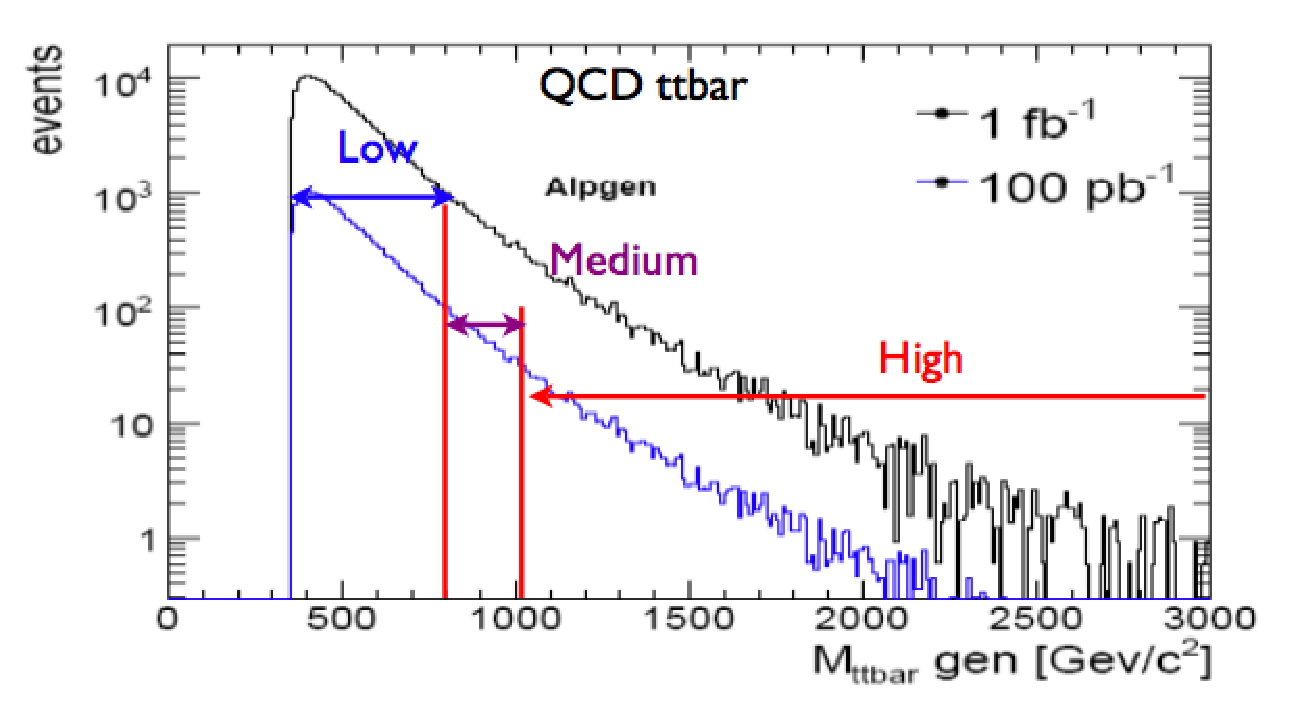
\includegraphics[width=0.8\textwidth]{fig05.ps}
\caption{Distribution of $m_{t\bar{t}}$ from generated QCD $t\bar{t}$ events using Alpgen for
1~$fb^{-1}$ and 100~$pb^{-1}$.}
\label{fig:fig5}
\end{figure}

\begin{figure}
\centering
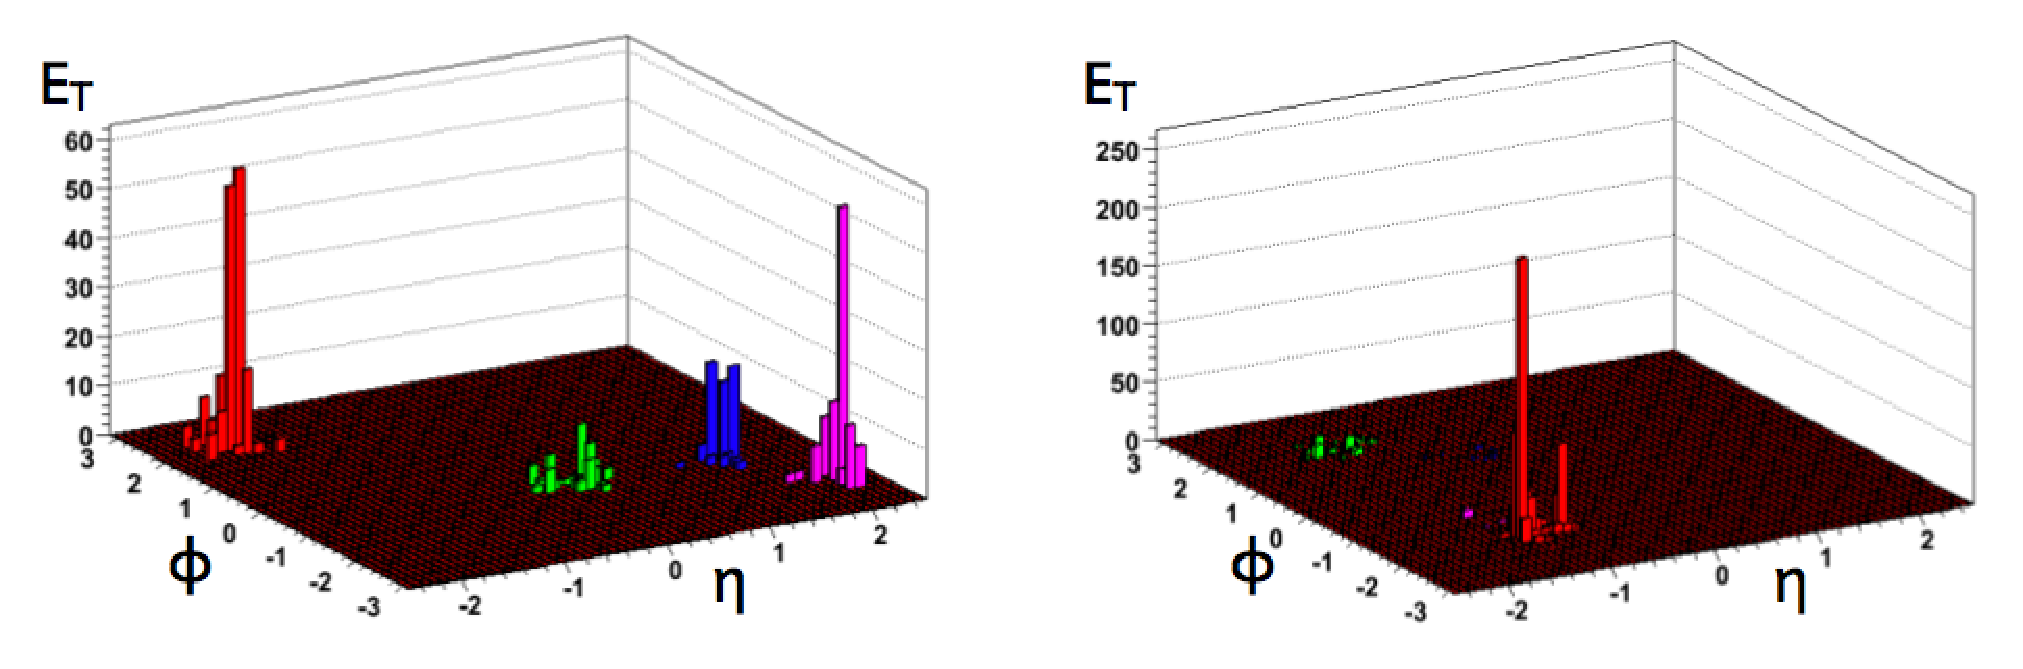
\includegraphics[width=1.1\textwidth]{fig07.ps}
\caption{Lego plot of the four leading calorimeter of an event from (a) QCD $t\bar{t}$ sample and (b) $Z'(4~TeV)\rightarrow t\bar{t}$ sample.}
\label{fig:fig7}
\end{figure}

\section{Conclusions}
\label{sec:Conclusions}

The LHC will open a very rich top-quark sector to look for new physics beyond the SM.
CMS has explored the discovery potential of BSM top quark decays like charged Higgs
bosons and FCNC decays. Analyses of several final state decays of $H^{+}$ have
been summarized in this note. These analyses are expected to be studied once the
detector and the SM backgrounds are well understood. The sensitivity contours for a sample
of 30~$fb^{-1}$ were presented. In the case of FCNC decays, the expected sensitivity
reach with 10~$fb^{-1}$ extends two order of magnitude larger than the Tevatron.
The search for heavy resonances decaying to top pairs is also being explored in CMS. The
top pair invariant mass is a good observable to carry on a model independent shape
search. CMS is studying different reconstruction techniques to improve the efficiency
of selecting boosted top jets.




\begin{thebibliography}{0}

\bibitem{ref:Wang} J.~Thaler and L.~T.~Wang,
%``Strategies to Identify Boosted Tops,''
  arXiv:0806.0023 [hep-ph].
%%CITATION = ARXIV:0806.0023;%%

\bibitem{ref:Han} T.~Han,
%``The 'Top Priority' at the LHC,''
  arXiv:0804.3178 [hep-ph].
%%CITATION = ARXIV:0804.3178;%%

\bibitem{ref:CMS} The CMS collaboration, \TITLE{The CMS Experiment at the CERN LHC},
Submitted to the Journal of Instrumentation, (2008).

\bibitem{ref:pdg} W.-M.Yao \etal (Particle Data Group), 
J. Phys. G 33, 1 (2006) and 2007 partial update for the 2008 edition.

\bibitem{ref:ptdr2} The CMS collaboration, \TITLE{Physics Technical Design Report, Volume II},
CERN/LHCC 2006-021.

\bibitem{ref:tauLepAna} M.~Baarmand, M.~Hashemi, and A.~Nikitenko, CMS Note 2006/056 (2006).

\bibitem{ref:jjtauAna}

\bibitem{ref:jetsAna} S.~Lowette, J.~D'Hondt, and P.~Vanlaer, CMS Note 2006/109 (2006).

\bibitem{ref:Maltoni} R.~Frederix and F.~Maltoni,
%``Top pair invariant mass distribution: a window on new physics,''
  arXiv:0712.2355 [hep-ph].
%%CITATION = ARXIV:0712.2355;%%

\bibitem{ref:other} L.~G.~Almeida, S.~J.~Lee, G.~Perez, G.~Sterman, I.~Sung and J.~Virzi,
  %``Substructure of high-p_T Jets at the LHC,''
  arXiv:0807.0234 [hep-ph].
  %%CITATION = ARXIV:0807.0234;%%

\end{thebibliography}

\end{document}
\endinput
%%
%% End of file `cimsmple.tex'.
